%----------------------------------------------------------------------------------------
%	PACKAGES AND OTHER DOCUMENT CONFIGURATIONS
%----------------------------------------------------------------------------------------

\documentclass[
	11pt, % Set the default font size, options include: 8pt, 9pt, 10pt, 11pt, 12pt, 14pt, 17pt, 20pt
	%t, % Uncomment to vertically align all slide content to the top of the slide, rather than the default centered
	%aspectratio=169, % Uncomment to set the aspect ratio to a 16:9 ratio which matches the aspect ratio of 1080p and 4K screens and projectors
]{beamer}

\graphicspath{{Images/}{./}}

\usepackage{booktabs}

\usetheme{Madrid}
\usecolortheme{orchid}
\usefonttheme{default} % Typeset using the default sans serif font

\usepackage{palatino} % Use the Palatino font for serif text
\usepackage[default]{opensans} % Use the Open Sans font for sans serif text

\useinnertheme{rectangles}

%\usepackage{styles/ngk813_style}

% ------------------------------------------------------------------------------
% Listings
% ------------------------------------------------------------------------------
\usepackage{textcomp}
\usepackage{listings}
\usepackage{inconsolata}
\usepackage{fontawesome} % egyedi listajelekhez például
\usepackage{graphicx}

\definecolor{mygreen}{HTML}{37980D}
\definecolor{myblue}{HTML}{0D089F}
\definecolor{myred}{HTML}{98290D}
\definecolor{mGreen}{rgb}{0,0.6,0}
\definecolor{mGray}{rgb}{0.5,0.5,0.5}
\definecolor{mPurple}{rgb}{0.58,0,0.82}
\definecolor{backgroundColour}{rgb}{0.98,0.98,0.98}

\newcommand{\quotetext}[1]{\begin{block}\footnotesize\textit{#1}\end{block}}

\newcommand{\sft}[1]{\section{#1}\frametitle{#1}\centering\LARGE#1}
\newcommand{\ssft}[1]{\subsection{#1}\frametitle{#1}}

\newcommand{\ascode}[1]{\textcolor{blue}{\fontfamily{DejaVu Sans Mono}\ttfamily\selectfont\replunderscores{#1}}}
\newcommand{\bfcode}[1]{\textbf{\ascode{#1}}}
\newcommand{\replunderscores}[1]{\expandafter\@repl@underscores#1_\relax}
\def\@repl@underscores#1_#2\relax{%
    \ifx \relax #2\relax
        % #2 is empty => finish
        #1%
    \else
        % #2 is not empty => underscore was contained, needs to be replaced
        #1%
        \textunderscore
        % continue replacing
        % #2 ends with an extra underscore so I don't need to add another one
        \@repl@underscores#2\relax
    \fi
}

\def\lstbasicfont{\fontfamily{DejaVu Sans Mono}\selectfont\footnotesize}

\lstset{%
basicstyle=\ttfamily
}
\lstdefinestyle{CStyle}{
    backgroundcolor=\color{backgroundColour},
    commentstyle=\color{mGreen},
    keywordstyle=\color{blue},
    numberstyle=\tiny\color{mGray},
    stringstyle=\color{mPurple},
    basicstyle=\footnotesize\ttfamily,
    breakatwhitespace=false,
    breaklines=true,
    captionpos=b,
    keepspaces=true,
    numbers=left,
    numbersep=5pt,
    showspaces=false,
    showstringspaces=false,
    showtabs=false,
    tabsize=4,
    language=C,
    xleftmargin=0.5cm,
    xrightmargin=0.5cm,
    upquote=true,
    inputencoding = utf8,  % Input encoding
    extendedchars = true,  % Extended ASCII
    literate      =        % Support additional characters
      {á}{{\'a}}1  {é}{{\'e}}1  {í}{{\'i}}1 {ó}{{\'o}}1  {ú}{{\'u}}1
      {Á}{{\'A}}1  {É}{{\'E}}1  {Í}{{\'I}}1 {Ó}{{\'O}}1  {Ú}{{\'U}}1
      {à}{{\`a}}1  {è}{{\`e}}1  {ì}{{\`i}}1 {ò}{{\`o}}1  {ù}{{\`u}}1
      {À}{{\`A}}1  {È}{{\'E}}1  {Ì}{{\`I}}1 {Ò}{{\`O}}1  {Ù}{{\`U}}1
      {ä}{{\"a}}1  {ë}{{\"e}}1  {ï}{{\"i}}1 {ö}{{\"o}}1  {ü}{{\"u}}1
      {ő}{{\~o}}1  {Ő}{{\~O}}1  {ű}{{\~u}}1 {Ű}{{\~U}}1
      {Ä}{{\"A}}1  {Ë}{{\"E}}1  {Ï}{{\"I}}1 {Ö}{{\"O}}1  {Ü}{{\"U}}1
      {â}{{\^a}}1  {ê}{{\^e}}1  {î}{{\^i}}1 {ô}{{\^o}}1  {û}{{\^u}}1
      {Â}{{\^A}}1  {Ê}{{\^E}}1  {Î}{{\^I}}1 {Ô}{{\^O}}1  {Û}{{\^U}}1
      {œ}{{\oe}}1  {Œ}{{\OE}}1  {æ}{{\ae}}1 {Æ}{{\AE}}1  {ß}{{\ss}}1
      {ç}{{\c c}}1 {Ç}{{\c C}}1 {ø}{{\o}}1  {Ø}{{\O}}1   {å}{{\r a}}1
      {Å}{{\r A}}1 {ã}{{\~a}}1  {õ}{{\~o}}1 {Ã}{{\~A}}1  {Õ}{{\~O}}1
      {ñ}{{\~n}}1  {Ñ}{{\~N}}1  {¿}{{?`}}1  {¡}{{!`}}1
      {°}{{\textdegree}}1 {º}{{\textordmasculine}}1 {ª}{{\textordfeminine}}1
      % ¿ and ¡ are not correctly displayed if inconsolata font is used
      % together with the lstlisting environment. Consider typing code in
      % external files and using \lstinputlisting to display them instead.
}

\lstdefinestyle{CMake}{
    backgroundcolor=\color{backgroundColour},
    commentstyle=\color{gray},
    numberstyle=\tiny\color{mGray},
    stringstyle=\color{mPurple},
    basicstyle=\footnotesize\ttfamily,
    breakatwhitespace=false,
    breaklines=true,
    captionpos=b,
    keepspaces=true,
    numbers=left,
    numbersep=5pt,
    showspaces=false,
    showstringspaces=false,
    showtabs=false,
    tabsize=4,
    language=bash,
    classoffset=0,
    morekeywords={cmake_minimum_required,project,include_directories,add_executable,CMAKE_RUNTIME_OUTPUT_DIRECTORY,CMAKE_BINARY_DIR,CMAKE_CURRENT_SOURCE_DIR},
    keywordstyle=\color{mGreen},
    classoffset=1,
    morekeywords={VERSION,},
    keywordstyle=\color{orange},
    classoffset=2,
    morekeywords={\$,\{,\}},
    keywordstyle=\color{myblue},
    xleftmargin=0.5cm,
    xrightmargin=0.5cm,
    upquote=true,
    inputencoding = utf8,  % Input encoding
    extendedchars = true,  % Extended ASCII
    literate      =        % Support additional characters
      {á}{{\'a}}1  {é}{{\'e}}1  {í}{{\'i}}1 {ó}{{\'o}}1  {ú}{{\'u}}1
      {Á}{{\'A}}1  {É}{{\'E}}1  {Í}{{\'I}}1 {Ó}{{\'O}}1  {Ú}{{\'U}}1
      {à}{{\`a}}1  {è}{{\`e}}1  {ì}{{\`i}}1 {ò}{{\`o}}1  {ù}{{\`u}}1
      {À}{{\`A}}1  {È}{{\'E}}1  {Ì}{{\`I}}1 {Ò}{{\`O}}1  {Ù}{{\`U}}1
      {ä}{{\"a}}1  {ë}{{\"e}}1  {ï}{{\"i}}1 {ö}{{\"o}}1  {ü}{{\"u}}1
      {ő}{{\~o}}1  {Ő}{{\~O}}1  {ű}{{\~u}}1 {Ű}{{\~U}}1
      {Ä}{{\"A}}1  {Ë}{{\"E}}1  {Ï}{{\"I}}1 {Ö}{{\"O}}1  {Ü}{{\"U}}1
      {â}{{\^a}}1  {ê}{{\^e}}1  {î}{{\^i}}1 {ô}{{\^o}}1  {û}{{\^u}}1
      {Â}{{\^A}}1  {Ê}{{\^E}}1  {Î}{{\^I}}1 {Ô}{{\^O}}1  {Û}{{\^U}}1
      {œ}{{\oe}}1  {Œ}{{\OE}}1  {æ}{{\ae}}1 {Æ}{{\AE}}1  {ß}{{\ss}}1
      {ç}{{\c c}}1 {Ç}{{\c C}}1 {ø}{{\o}}1  {Ø}{{\O}}1   {å}{{\r a}}1
      {Å}{{\r A}}1 {ã}{{\~a}}1  {õ}{{\~o}}1 {Ã}{{\~A}}1  {Õ}{{\~O}}1
      {ñ}{{\~n}}1  {Ñ}{{\~N}}1  {¿}{{?`}}1  {¡}{{!`}}1
      {°}{{\textdegree}}1 {º}{{\textordmasculine}}1 {ª}{{\textordfeminine}}1
      % ¿ and ¡ are not correctly displayed if inconsolata font is used
      % together with the lstlisting environment. Consider typing code in
      % external files and using \lstinputlisting to display them instead.
}

%----------------------------------------------------------------------------------------
%	PRESENTATION INFORMATION
%----------------------------------------------------------------------------------------

\title[Linux kernel and C programming]{Linux kernel and C programming}
\subtitle{BLOCK 1: Introduction to Memory}
\author[Gergely Korcsák]{Gergely Korcsák}
\institute[OE NIK]{Óbuda University \\ \smallskip \textit{korcsak.gergely@nik.uni-obuda.hu}}
\date[\today]{\today}

%----------------------------------------------------------------------------------------

\begin{document}

%----------------------------------------------------------------------------------------
%	TITLE SLIDE
%----------------------------------------------------------------------------------------

\begin{frame}
	\titlepage
\end{frame}

%----------------------------------------------------------------------------------------
%	TABLE OF CONTENTS SLIDE
%----------------------------------------------------------------------------------------

\begin{frame}
	\frametitle{Presentation Overview} % Slide title, remove this command for no title

	\tableofcontents % Output the table of contents (all sections on one slide)
    %\tableofcontents[pausesections,sections={1}] % Output the table of contents (break sections up across separate slides)
\end{frame}

%----------------------------------------------------------------------------------------
%	PRESENTATION BODY SLIDES
%----------------------------------------------------------------------------------------

\begin{frame}
    \sft{Memory}
\end{frame}

\begin{frame}
    \ssft{Memory Types}

    \centering
    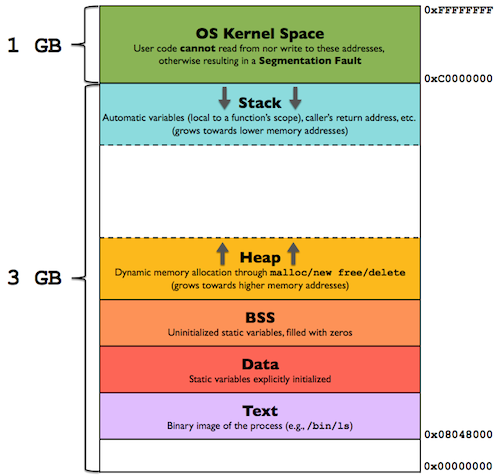
\includegraphics[width=.7\linewidth]{images/program_in_memory.png}
\end{frame}

\begin{frame}
    \ssft{Program}

    \begin{block}{Program memory}
        Stores the program (\ascode{text}) data.
        Which is the executable software.
    \end{block}
\end{frame}

\begin{frame}
    \ssft{Data}

    \begin{exampleblock}{Runtime}
        The state of a program when it starts executing the main function.
    \end{exampleblock}

    \bigskip
    \begin{block}{Data memory}
        Stores the constant and static variables, that are initialized before runtime.
        These are usually default configs, and parameters, like memory addresses of components (eg: uart driver address map).
    \end{block}

    \bigskip
    \begin{block}{BSS memory}
        Stores zeroed variables, which have a specific size, and initialized before runtime.
    \end{block}
\end{frame}

\begin{frame}
    \ssft{Heap}

    \begin{block}{Heap}
        The heap stores every variable which has been allocated during runtime.
    \end{block}

    \bigskip
    \begin{alertblock}{Alert}
        In the user-space every application memory will be freed, after the program execution,
        but in kernel-space, the memory will only be freed by ether using the \ascode{free} operator or
        restarting the system.
    \end{alertblock}
\end{frame}

\begin{frame}
    \ssft{Stack}

    \begin{block}{Stack}
        The stack is a constantly changing memory, where every new function variable will be allocated.
        The growth direction of the stack is dependent on the system, but usually it grows downwards, by every new function call.
        If a function is executed, and returned, the stack location is freed.
    \end{block}

    \bigskip
    \begin{exampleblock}{Stack overflow?}
        Stack overflow is when we fill up the stack and start to use memory areas that are not meant to be used as
        function variable area.
        Therefore it can cause execution errors.

        Like not returning from a recursive function, before reaching the stack size.
    \end{exampleblock}
\end{frame}

\begin{frame}
    \ssft{Stack protection}

    \begin{alertblock}{Be aware}
        As the stack is for functions, it also contains the return addresses. To where the current function will return
        after its execution is finished.
        If the stack becomes corrupted by some unchecked memory fill. An "attacker" can modify the return address,
        To point to their own code.
    \end{alertblock}

    \bigskip
    \begin{exampleblock}{Stack canary}
        There are several stack and return protection features in modern hardware and software, but by default it is
        usually turned off.
        We can use stack canaries, to add an extra word of memory into the end of a functions allocated stack,
        so if we overflow it, it will cause an error.
    \end{exampleblock}
\end{frame}

\begin{frame}
    \sft{Memory allocation}
\end{frame}

\begin{frame}[fragile]
    \ssft{User-space malloc}

    In user-space we can allocate memory (\textbf{from the Heap}) by calling the \ascode{malloc()} function.

    It will only need a memory size in bytes, and will return a void pointer, to the newly allocated memory.
    If it fails, it will return 0.

    \begin{lstlisting}[style=CStyle]
// Will allocate 12 bytes of memory
int* array1 = (int*)malloc(12);
// Will allocate 4x12 bytes of memory
int* array2 = (int*)malloc(sizeof(int) * 12);

struct person {
    char* name;
    int age;
};
// Will allocate 12 bytes of memory
struct person* myperson =
    (struct person*)malloc(sizeof(struct person));

\end{lstlisting}
\end{frame}

\begin{frame}[fragile]
    \ssft{User-space free}

    After we allocate an area, it will not be reallocated to another variables and programs, until it is freed.
    We can free up an allocated memory area by calling the \ascode{free()} function.

    \begin{lstlisting}[style=CStyle]
// Will allocate 40 bytes of memory
int* array = (int*)malloc(sizeof(int) * 10);

// some array manipulation here..

// Will free up 40 bytes of memory
free(array);

\end{lstlisting}

    \bigskip
    \begin{alertblock}{User after free}
        If we would use the previously allocated then freed variable again, it would be "use after free",
        which can cause undefined behavior.
    \end{alertblock}
\end{frame}

\begin{frame}[fragile]
    \ssft{Kernel-space}

    We can also allocate and free memory in the kernel when programming modules, but using \ascode{kmalloc} and \ascode{kfree}:

    \begin{lstlisting}[style=CStyle]
// in linux/slab.h
void* kmalloc(size_t size, int flags);
void kfree(void* obj)

\end{lstlisting}

    The \ascode{flags} will be used to decide the type of memory to be allocated.

    \begin{table}[h]
        \centering
        \begin{tabular}{|p{.2\textwidth}|p{.5\textwidth}|}
            \hline
            \textbf{Flag}       & \textbf{Description}                              \\
            \hline
            \ascode{GFP_USER}   & Allocate memory on behalf of user. (may sleep)    \\
            \ascode{GFP_KERNEL} & Allocate normal kernel memory. (may sleep)        \\
            \ascode{GFP_ATOMIC} & Allocation will not sleep. (use in interrupts)    \\
            \ascode{GFP_NOWAIT} & Allocation will not sleep.                        \\
            ...                 & ...                                               \\
            \hline

        \end{tabular}
    \end{table}

\end{frame}

\begin{frame}
    \sft{Strings}
\end{frame}

\begin{frame}
    \ssft{String functions}

    Some string functions are basically \ascode{memcpy()}, but will use the \ascode{'\\0'} character as size.

    \begin{table}[h]
        \centering
        \begin{tabular}{|p{.4\textwidth}|p{.5\textwidth}|}
            \hline
            \textbf{Function}               & \textbf{Description}                                                  \\
            \hline \ascode{strlen(str)}            & Will return the string length, excluding the \ascode{'\textbackslash0'} character. \\
            \hline \ascode{strcpy(dest, src)}      & Will copy \ascode{src} to \ascode{dest}. \\
            \hline \ascode{strncpy(dest, src, n)}  & Will copy n characters from \ascode{src} to \ascode{dest}. \\
            \hline \ascode{strcat(dest, src)}      & Concatenate \ascode{src} to the end of \ascode{dest}. \\
            \hline \ascode{strncat(dest, src, n)}  & Concatenate n characters from \ascode{src} to the end of \ascode{dest}. \\
            \hline \ascode{strcmp(dest, src)}      & Compares \ascode{src} to \ascode{dest}. \\
            \hline \ascode{strncmp(dest, src, n)}  & Compares n characters from \ascode{src} to \ascode{dest}. \\
            \hline

        \end{tabular}
    \end{table}

\end{frame}
\begin{frame}[fragile]
    \frametitle{String functions}

    Some string functions are basically \ascode{memcpy()}, but will use the \ascode{'\\0'} character as size.

    \begin{table}[h]
        \centering
        \begin{tabular}{|p{.4\textwidth}|p{.5\textwidth}|}
            \hline
            \textbf{Function}               & \textbf{Description}                                                  \\
            \hline \ascode{strchar(str, c)}        & Find the first occurrence of 'c' or return NULL.  \\
            \hline \ascode{strrchar(str, c)}       & Find the last occurrence of 'c' or return NULL.  \\
            \hline \ascode{strstr(str, sub)}       & Find the first occurrence of the sub-string or return NULL.  \\
            \hline

        \end{tabular}
    \end{table}

    \bigskip
    We can also use \ascode{sprintf()} to print into an allocated memory area, instead of the standard output.

    \begin{lstlisting}[style=CStyle]
char* fname = "Balu";
char* lname = "Hasu";
char name[100] = { 0 };
sprintf(name, "Name is: %s %s", fname, lname);
printf("name: %s\n", name);

\end{lstlisting}

\end{frame}

\begin{frame}
    \sft{"Safe" functions}
\end{frame}

\begin{frame}
    \sft{Exercises}
\end{frame}

\begin{frame}[fragile]
    \frametitle{Exercises}

    Declare the following functions:

    \begin{lstlisting}[style=CStyle]
#ifndef __MALLOC_H__
#define __MALLOC_H__

#include <stdint.h>

#define MALLOC_BUF_SIZE 0x1000U
#define BEEF            0xBEEFBEEF
#define NULL            0x0U

struct allocator {
    uint32_t beef;
    uint32_t size;
};

void*   my_malloc(unsigned long long size);
int     my_free(void* obj);

#endif /* __MALLOC_H__ */

\end{lstlisting}

\end{frame}

%----------------------------------------------------------------------------------------
%	CLOSING SLIDE
%----------------------------------------------------------------------------------------

\begin{frame}[plain] % The optional argument 'plain' hides the headline and footline
	\begin{center}
		{\Huge The End}

		\bigskip\bigskip % Vertical whitespace

		{\LARGE Questions? Comments?}
	\end{center}
\end{frame}

%----------------------------------------------------------------------------------------

\end{document}
